% Figure F3_heatmap_model_variant of study_analysis_001 - generated by thesis/study_analysis/figures.py; do not edit by hand.
% Preamble: \usepackage{pgfplots}
%           \pgfplotsset{compat=1.18}
% Net correctness gain per model and variant (R04, Q06)
% Caption: figures/F3_heatmap_model_variant.caption.tex (figure_caption_tex)
% Composite block; cell = R04 net gain of Q06 correctness pass (FINAL[v] - BASE) in percentage points; blue = gain, red = loss, gray midpoint = 0 (colour scale beside the plot); bold value = its 95% CI excludes 0 (a degenerate zero-width interval is never bold; its value carries †); descriptive per model (unadjusted CIs, no test, no ranking)
% CIs (in the data CSV): 95% CI: nonparametric cluster bootstrap, percentile intervals, stratified by block (pilot benchmarks resampled among the 12 pilot benchmarks, full_ext among its 48); seed 20261017; cluster = benchmark; 2,000 replicates (descriptive, unadjusted)
% BL01: Includes dense_la/00 (BL-01 tolerance convention: possible false FAIL verdicts; disclosure-bearing aggregate); sensitivity SA1 in T10.
% REASONING: Reasoning settings differ between models and are not equalised (see the closure disclosure register, item reasoning_policy_differences); some providers report no reasoning-token field.
% IC1: Q06 is in-sample for test_feedback and combined_feedback: their loops see the ParEval test verdict and stop when it passes (every stopped_tests_pass trajectory is a Q06 pass), so they optimise the endpoint; for static_feedback Q06 is out-of-sample (measured once in phase 2, never seen by the loop). The variants therefore differ in trigger and stop rules, not only in feedback content; test_feedback cannot regress on Q06 by construction.
% IC2: E02 is not an independent confirmation of Q06 gains: it counts build failures, and most E02 improvements are the same cells as the Q06 improvements; the held-out signal proper is the joint transition X06 (e.g. Q06 repaired but E02 still failing) and G01.
% IC6: static_feedback repair triggers are dominated by clang-tidy bugprone findings and, on MPI, by low-confidence hints (design document: no trustworthy static MPI tool exists); static_feedback results measure this frozen blocking-set configuration, not static analysis in general.
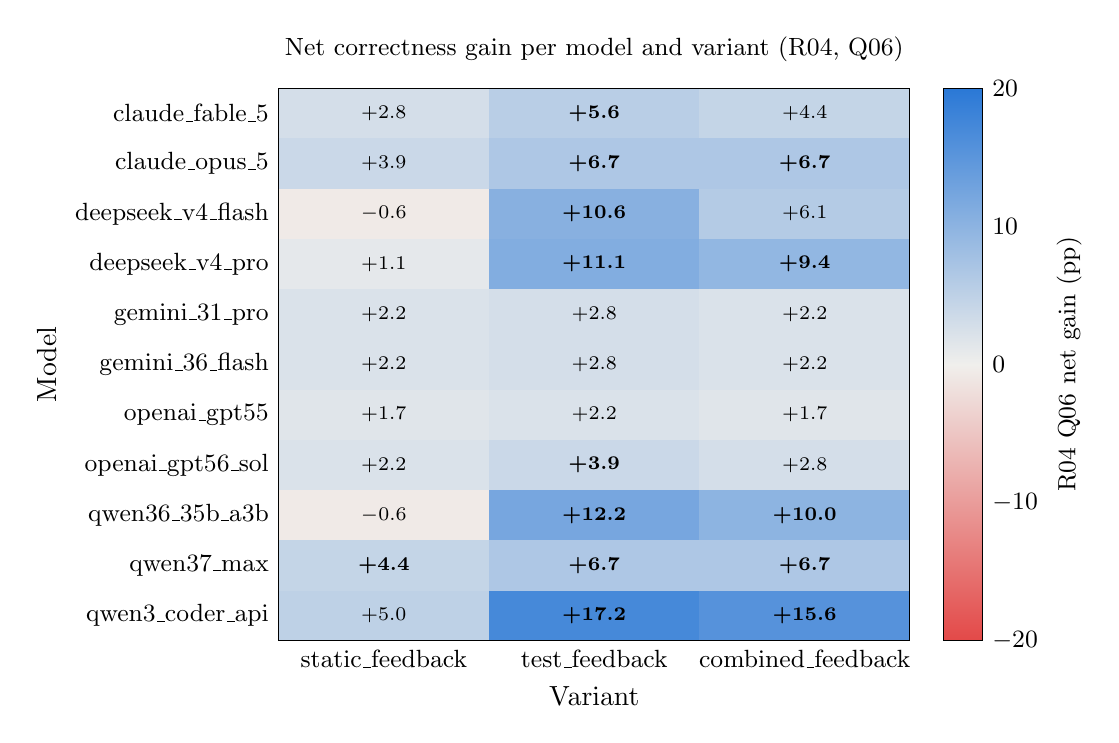
\begin{tikzpicture}
\definecolor{saHeat0}{HTML}{D4DEE9}
\definecolor{saHeat1}{HTML}{B9CEE6}
\definecolor{saHeat2}{HTML}{C4D5E7}
\definecolor{saHeat3}{HTML}{CAD8E8}
\definecolor{saHeat4}{HTML}{AEC7E5}
\definecolor{saHeat5}{HTML}{AEC7E5}
\definecolor{saHeat6}{HTML}{F0EAE7}
\definecolor{saHeat7}{HTML}{88B0E0}
\definecolor{saHeat8}{HTML}{B4CBE5}
\definecolor{saHeat9}{HTML}{E5E8EB}
\definecolor{saHeat10}{HTML}{82ADE0}
\definecolor{saHeat11}{HTML}{92B7E2}
\definecolor{saHeat12}{HTML}{DAE2EA}
\definecolor{saHeat13}{HTML}{D4DEE9}
\definecolor{saHeat14}{HTML}{DAE2EA}
\definecolor{saHeat15}{HTML}{DAE2EA}
\definecolor{saHeat16}{HTML}{D4DEE9}
\definecolor{saHeat17}{HTML}{DAE2EA}
\definecolor{saHeat18}{HTML}{E0E5EA}
\definecolor{saHeat19}{HTML}{DAE2EA}
\definecolor{saHeat20}{HTML}{E0E5EA}
\definecolor{saHeat21}{HTML}{DAE2EA}
\definecolor{saHeat22}{HTML}{CAD8E8}
\definecolor{saHeat23}{HTML}{D4DEE9}
\definecolor{saHeat24}{HTML}{F0EAE7}
\definecolor{saHeat25}{HTML}{77A6DF}
\definecolor{saHeat26}{HTML}{8DB4E1}
\definecolor{saHeat27}{HTML}{C4D5E7}
\definecolor{saHeat28}{HTML}{AEC7E5}
\definecolor{saHeat29}{HTML}{AEC7E5}
\definecolor{saHeat30}{HTML}{BED1E6}
\definecolor{saHeat31}{HTML}{4689D9}
\definecolor{saHeat32}{HTML}{5692DB}
\begin{axis}[
  width=9.600cm,
  height=8.600cm,
  xmin=-0.5,
  xmax=2.500,
  ymin=-0.5,
  ymax=10.500,
  y dir=reverse,
  axis on top,
  tick style={draw=none},
  xtick={0,1,2},
  xticklabels={{static\_feedback},{test\_feedback},{combined\_feedback}},
  ytick={0,1,2,3,4,5,6,7,8,9,10},
  yticklabels={{claude\_fable\_5},{claude\_opus\_5},{deepseek\_v4\_flash},{deepseek\_v4\_pro},{gemini\_31\_pro},{gemini\_36\_flash},{openai\_gpt55},{openai\_gpt56\_sol},{qwen36\_35b\_a3b},{qwen37\_max},{qwen3\_coder\_api}},
  xlabel={Variant},
  ylabel={Model},
  x tick label style={font=\small},
  y tick label style={font=\small},
  colormap={saDiverging}{rgb255=(227,73,72) rgb255=(240,239,236) rgb255=(42,120,214)},
  colorbar,
  point meta min=-20.000,
  point meta max=20.000,
  colorbar style={ylabel={R04 Q06 net gain (pp)}, font=\small},
  title={Net correctness gain per model and variant (R04, Q06)},
  title style={font=\small}
]
\addplot[draw=none, mark=none, forget plot] coordinates {(-0.5,-0.5) (2.500,10.500)};
\fill[saHeat0] (axis cs:-0.500,-0.500) rectangle (axis cs:0.500,0.500);
\node[font=\scriptsize, text=black] at (axis cs:0,0) {+2.8};
\fill[saHeat1] (axis cs:0.500,-0.500) rectangle (axis cs:1.500,0.500);
\node[font=\scriptsize, text=black] at (axis cs:1,0) {\textbf{+5.6}};
\fill[saHeat2] (axis cs:1.500,-0.500) rectangle (axis cs:2.500,0.500);
\node[font=\scriptsize, text=black] at (axis cs:2,0) {+4.4};
\fill[saHeat3] (axis cs:-0.500,0.500) rectangle (axis cs:0.500,1.500);
\node[font=\scriptsize, text=black] at (axis cs:0,1) {+3.9};
\fill[saHeat4] (axis cs:0.500,0.500) rectangle (axis cs:1.500,1.500);
\node[font=\scriptsize, text=black] at (axis cs:1,1) {\textbf{+6.7}};
\fill[saHeat5] (axis cs:1.500,0.500) rectangle (axis cs:2.500,1.500);
\node[font=\scriptsize, text=black] at (axis cs:2,1) {\textbf{+6.7}};
\fill[saHeat6] (axis cs:-0.500,1.500) rectangle (axis cs:0.500,2.500);
\node[font=\scriptsize, text=black] at (axis cs:0,2) {$-$0.6};
\fill[saHeat7] (axis cs:0.500,1.500) rectangle (axis cs:1.500,2.500);
\node[font=\scriptsize, text=black] at (axis cs:1,2) {\textbf{+10.6}};
\fill[saHeat8] (axis cs:1.500,1.500) rectangle (axis cs:2.500,2.500);
\node[font=\scriptsize, text=black] at (axis cs:2,2) {+6.1};
\fill[saHeat9] (axis cs:-0.500,2.500) rectangle (axis cs:0.500,3.500);
\node[font=\scriptsize, text=black] at (axis cs:0,3) {+1.1};
\fill[saHeat10] (axis cs:0.500,2.500) rectangle (axis cs:1.500,3.500);
\node[font=\scriptsize, text=black] at (axis cs:1,3) {\textbf{+11.1}};
\fill[saHeat11] (axis cs:1.500,2.500) rectangle (axis cs:2.500,3.500);
\node[font=\scriptsize, text=black] at (axis cs:2,3) {\textbf{+9.4}};
\fill[saHeat12] (axis cs:-0.500,3.500) rectangle (axis cs:0.500,4.500);
\node[font=\scriptsize, text=black] at (axis cs:0,4) {+2.2};
\fill[saHeat13] (axis cs:0.500,3.500) rectangle (axis cs:1.500,4.500);
\node[font=\scriptsize, text=black] at (axis cs:1,4) {+2.8};
\fill[saHeat14] (axis cs:1.500,3.500) rectangle (axis cs:2.500,4.500);
\node[font=\scriptsize, text=black] at (axis cs:2,4) {+2.2};
\fill[saHeat15] (axis cs:-0.500,4.500) rectangle (axis cs:0.500,5.500);
\node[font=\scriptsize, text=black] at (axis cs:0,5) {+2.2};
\fill[saHeat16] (axis cs:0.500,4.500) rectangle (axis cs:1.500,5.500);
\node[font=\scriptsize, text=black] at (axis cs:1,5) {+2.8};
\fill[saHeat17] (axis cs:1.500,4.500) rectangle (axis cs:2.500,5.500);
\node[font=\scriptsize, text=black] at (axis cs:2,5) {+2.2};
\fill[saHeat18] (axis cs:-0.500,5.500) rectangle (axis cs:0.500,6.500);
\node[font=\scriptsize, text=black] at (axis cs:0,6) {+1.7};
\fill[saHeat19] (axis cs:0.500,5.500) rectangle (axis cs:1.500,6.500);
\node[font=\scriptsize, text=black] at (axis cs:1,6) {+2.2};
\fill[saHeat20] (axis cs:1.500,5.500) rectangle (axis cs:2.500,6.500);
\node[font=\scriptsize, text=black] at (axis cs:2,6) {+1.7};
\fill[saHeat21] (axis cs:-0.500,6.500) rectangle (axis cs:0.500,7.500);
\node[font=\scriptsize, text=black] at (axis cs:0,7) {+2.2};
\fill[saHeat22] (axis cs:0.500,6.500) rectangle (axis cs:1.500,7.500);
\node[font=\scriptsize, text=black] at (axis cs:1,7) {\textbf{+3.9}};
\fill[saHeat23] (axis cs:1.500,6.500) rectangle (axis cs:2.500,7.500);
\node[font=\scriptsize, text=black] at (axis cs:2,7) {+2.8};
\fill[saHeat24] (axis cs:-0.500,7.500) rectangle (axis cs:0.500,8.500);
\node[font=\scriptsize, text=black] at (axis cs:0,8) {$-$0.6};
\fill[saHeat25] (axis cs:0.500,7.500) rectangle (axis cs:1.500,8.500);
\node[font=\scriptsize, text=black] at (axis cs:1,8) {\textbf{+12.2}};
\fill[saHeat26] (axis cs:1.500,7.500) rectangle (axis cs:2.500,8.500);
\node[font=\scriptsize, text=black] at (axis cs:2,8) {\textbf{+10.0}};
\fill[saHeat27] (axis cs:-0.500,8.500) rectangle (axis cs:0.500,9.500);
\node[font=\scriptsize, text=black] at (axis cs:0,9) {\textbf{+4.4}};
\fill[saHeat28] (axis cs:0.500,8.500) rectangle (axis cs:1.500,9.500);
\node[font=\scriptsize, text=black] at (axis cs:1,9) {\textbf{+6.7}};
\fill[saHeat29] (axis cs:1.500,8.500) rectangle (axis cs:2.500,9.500);
\node[font=\scriptsize, text=black] at (axis cs:2,9) {\textbf{+6.7}};
\fill[saHeat30] (axis cs:-0.500,9.500) rectangle (axis cs:0.500,10.500);
\node[font=\scriptsize, text=black] at (axis cs:0,10) {+5.0};
\fill[saHeat31] (axis cs:0.500,9.500) rectangle (axis cs:1.500,10.500);
\node[font=\scriptsize, text=black] at (axis cs:1,10) {\textbf{+17.2}};
\fill[saHeat32] (axis cs:1.500,9.500) rectangle (axis cs:2.500,10.500);
\node[font=\scriptsize, text=black] at (axis cs:2,10) {\textbf{+15.6}};
\end{axis}
\end{tikzpicture}
